\documentclass[tikz,border=6pt]{standalone}
\usepackage[T1]{fontenc}
\usepackage[scaled=0.92]{helvet}
\usepackage{amsmath,amssymb}
\usepackage{tikz}
\usetikzlibrary{arrows.meta,positioning,shapes.geometric,shapes.misc,calc,fit,backgrounds}

\begin{document}
\sffamily
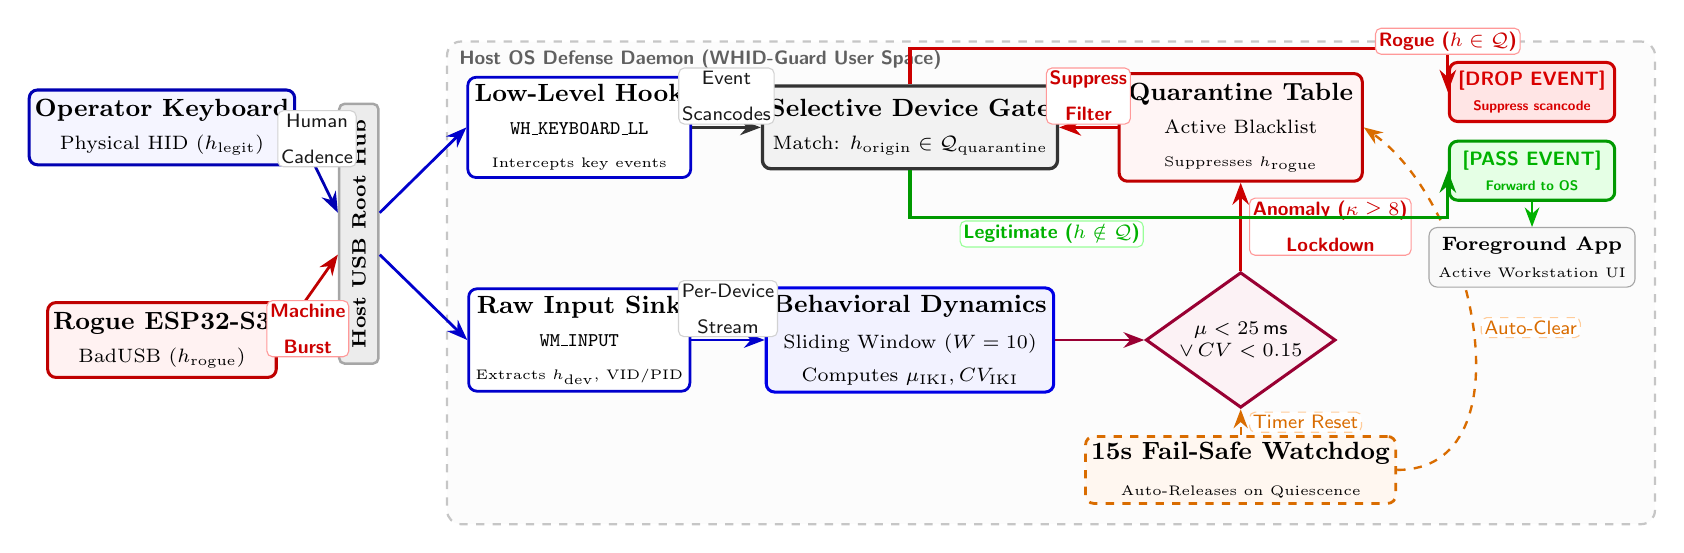
\begin{tikzpicture}[
    >=Stealth,
    font=\small,
    % Device blocks
    dev_rogue/.style={
        rectangle,
        rounded corners=3pt,
        draw=red!75!black,
        line width=1.1pt,
        fill=red!5!white,
        minimum width=2.2cm,
        minimum height=0.95cm,
        inner sep=2pt,
        align=center
    },
    dev_legit/.style={
        rectangle,
        rounded corners=3pt,
        draw=blue!70!black,
        line width=1.1pt,
        fill=blue!4!white,
        minimum width=2.2cm,
        minimum height=0.95cm,
        inner sep=2pt,
        align=center
    },
    % Module block
    mod_block/.style={
        rectangle,
        rounded corners=3pt,
        draw=blue!80!black,
        line width=1.0pt,
        fill=white,
        minimum width=2.2cm,
        minimum height=1.05cm,
        inner sep=2.5pt,
        align=center
    },
    % Engine block
    eng_block/.style={
        rectangle,
        rounded corners=3pt,
        draw=blue!90!black,
        line width=1.1pt,
        fill=blue!5!white,
        minimum width=2.5cm,
        minimum height=1.15cm,
        inner sep=2.5pt,
        align=center
    },
    % Decision Diamond
    decision/.style={
        diamond,
        aspect=1.4,
        draw=purple!80!black,
        line width=1.1pt,
        fill=purple!5!white,
        inner sep=1.2pt,
        align=center,
        font=\sffamily\scriptsize
    },
    % Gate switch
    gate_block/.style={
        rectangle,
        rounded corners=3pt,
        draw=black!80,
        line width=1.2pt,
        fill=gray!10!white,
        minimum width=2.4cm,
        minimum height=1.05cm,
        inner sep=2.5pt,
        align=center
    },
    % Action pills
    pill_drop/.style={
        rectangle,
        rounded corners=3pt,
        draw=red!80!black,
        line width=1.1pt,
        fill=red!10!white,
        minimum width=2.1cm,
        minimum height=0.75cm,
        inner sep=2pt,
        align=center,
        font=\sffamily\scriptsize\bfseries,
        text=red!85!black
    },
    pill_pass/.style={
        rectangle,
        rounded corners=3pt,
        draw=green!60!black,
        line width=1.1pt,
        fill=green!10!white,
        minimum width=2.1cm,
        minimum height=0.75cm,
        inner sep=2pt,
        align=center,
        font=\sffamily\scriptsize\bfseries,
        text=green!70!black
    },
    % Watchdog
    wdt_block/.style={
        rectangle,
        rounded corners=3pt,
        draw=orange!85!black,
        line width=1.0pt,
        dashed,
        fill=orange!6!white,
        minimum width=2.3cm,
        minimum height=0.85cm,
        inner sep=2pt,
        align=center
    },
    % Badges with tight padding
    lbl/.style={
        font=\sffamily\scriptsize,
        fill=white,
        draw=gray!35,
        line width=0.4pt,
        rounded corners=2pt,
        inner sep=1.2pt,
        align=center,
        text=black!90
    },
    lbl_red/.style={
        font=\sffamily\scriptsize\bfseries,
        fill=white,
        draw=red!40,
        line width=0.4pt,
        rounded corners=2pt,
        inner sep=1.2pt,
        align=center,
        text=red!80!black
    },
    lbl_green/.style={
        font=\sffamily\scriptsize\bfseries,
        fill=white,
        draw=green!40,
        line width=0.4pt,
        rounded corners=2pt,
        inner sep=1.2pt,
        align=center,
        text=green!70!black
    },
    lbl_amber/.style={
        font=\sffamily\scriptsize,
        fill=white,
        draw=orange!40,
        line width=0.4pt,
        rounded corners=2pt,
        inner sep=1.2pt,
        align=center,
        text=orange!85!black
    }
]

% ==============================================================================
% Column 1: Physical Peripherals (x = 1.1)
% ==============================================================================
\node[dev_legit] (kb_legit) at (1.1, 1.35) {\textbf{Operator Keyboard}\\[1pt]\scriptsize Physical HID ($h_{\text{legit}}$)};
\node[dev_rogue] (badusb)   at (1.1, -1.35) {\textbf{Rogue ESP32-S3}\\[1pt]\scriptsize BadUSB ($h_{\text{rogue}}$)};

% Column 2: Host USB Bus (x = 3.6)
\node[rectangle, draw=gray!70, fill=gray!15, line width=0.9pt, minimum width=0.5cm, minimum height=3.3cm, rounded corners=2pt, align=center] (bus) at (3.6, 0) {\rotatebox{90}{\scriptsize\textbf{Host USB Root Hub}}};

\draw[->, line width=1.0pt, draw=blue!70!black] (kb_legit.east) -- node[above=1pt, lbl] {Human\\[5pt]Cadence} (bus.135);
\draw[->, line width=1.0pt, draw=red!75!black]  (badusb.east)   -- node[below=1pt, lbl_red] {Machine\\[5pt]Burst} (bus.225);

% ==============================================================================
% Column 3: Ingestion Dual Channels (x = 6.4)
% ==============================================================================
% Channel A: Low-Level Hook (Top Pipeline)
\node[mod_block] (hook) at (6.4, 1.35) {\textbf{Low-Level Hook}\\[1pt]\scriptsize \texttt{WH\_KEYBOARD\_LL}\\[1pt]\tiny Intercepts key events};

% Channel B: Raw Input Telemetry (Bottom Pipeline)
\node[mod_block] (rawinput) at (6.4, -1.35) {\textbf{Raw Input Sink}\\[1pt]\scriptsize \texttt{WM\_INPUT}\\[1pt]\tiny Extracts $h_{\text{dev}}$, VID/PID};

\draw[->, line width=1.0pt, draw=blue!80!black] (bus.45) -- (hook.west);
\draw[->, line width=1.0pt, draw=blue!80!black] (bus.315) -- (rawinput.west);

% ==============================================================================
% Column 4: Processing Modules (x = 10.6)
% ==============================================================================
% Top: Selective Device Gate
\node[gate_block] (gate) at (10.6, 1.35) {\textbf{Selective Device Gate}\\[1pt]\scriptsize Match: $h_{\text{origin}} \in \mathcal{Q}_{\text{quarantine}}$};
\draw[->, line width=1.0pt, draw=black!80] (hook.east) -- node[above=1pt, lbl] {Event\\[5pt]Scancodes} (gate.west);

% Bottom: Behavioral Dynamics Engine
\node[eng_block] (engine) at (10.6, -1.35) {\textbf{Behavioral Dynamics}\\[2pt]\scriptsize Sliding Window ($W=10$)\\[1pt]\scriptsize Computes $\mu_{\text{IKI}}, CV_{\text{IKI}}$};
\draw[->, line width=1.0pt, draw=blue!80!black] (rawinput.east) -- node[above=1pt, lbl] {Per-Device\\[5pt]Stream} (engine.west);

% ==============================================================================
% Column 5: Quarantine Table & Classification (x = 14.8)
% ==============================================================================
% Top: Quarantine State Table
\node[rectangle, rounded corners=3pt, draw=red!75!black, line width=1.1pt, fill=red!4!white, minimum width=2.3cm, minimum height=1.05cm, align=center] (qset) at (14.8, 1.35) {\textbf{Quarantine Table}\\[1pt]\scriptsize Active Blacklist\\[1pt]\tiny Suppresses $h_{\text{rogue}}$};

% Bottom: Decision Boundary Diamond
\node[decision] (decision_box) at (14.8, -1.35) {$\mu < 25\,\text{ms}$\\$\lor\,CV < 0.15$};
\draw[->, line width=1.0pt, draw=purple!80!black] (engine.east) -- (decision_box.west);

% Vertical Quarantine update from Decision Diamond to Q-Set
\draw[->, line width=1.1pt, draw=red!80!black] (decision_box.north) -- node[pos=0.50, right=3pt, lbl_red] {Anomaly ($\kappa \ge 8$)\\[5pt]Lockdown} (qset.south);

% Feeding Q-Set into Gate
\draw[->, line width=1.1pt, draw=red!80!black] (qset.west) -- node[above=1pt, lbl_red] {Suppress\\[5pt]Filter} (gate.east);

% Fail-Safe Watchdog (Below Decision Box, y = -3.00)
\node[wdt_block] (wdt) at (14.8, -3.00) {\textbf{15s Fail-Safe Watchdog}\\[2pt]\tiny Auto-Releases on Quiescence};
\draw[->, line width=0.85pt, dashed, draw=orange!85!black] (wdt.north) -- node[right=3pt, lbl_amber] {Timer Reset} (decision_box.south);
\draw[->, line width=0.85pt, dashed, draw=orange!85!black] (wdt.east) to[out=0, in=-35] node[pos=0.5, right=3pt, lbl_amber] {Auto-Clear} (qset.east);

% ==============================================================================
% Column 6: Dual Enforcement Outputs (x = 18.5)
% ==============================================================================
\node[pill_drop] (drop_out) at (18.5, 1.8) {\textbf{[DROP EVENT]}\\[1pt]\tiny Suppress scancode};
\node[pill_pass] (pass_out) at (18.5, 0.8) {\textbf{[PASS EVENT]}\\[1pt]\tiny Forward to OS};

% Routing from Gate to Outputs
\draw[->, line width=1.1pt, draw=red!80!black] (gate.north) -- ++(0, 0.45) -| node[pos=0.6, above=1pt, lbl_red] {Rogue ($h \in \mathcal{Q}$)} (drop_out.west);
\draw[->, line width=1.1pt, draw=green!60!black] (gate.south) -- ++(0, -0.6) -- ++(1.8, 0) node[below=1pt, lbl_green] {Legitimate ($h \notin \mathcal{Q}$)} -| (pass_out.west);

% Target OS Application Focus Box
\node[rectangle, rounded corners=3pt, draw=gray!70, fill=gray!5, minimum width=2.2cm, minimum height=0.75cm, align=center] (target_app) at (18.5, -0.3) {\scriptsize\textbf{Foreground App}\\[-1pt]\tiny Active Workstation UI};

\draw[->, line width=0.9pt, draw=green!70!black] (pass_out.south) -- (target_app.north);

% Background Container: Host OS User Space
\begin{scope}[on background layer]
    \node[rectangle, draw=gray!45, dashed, fill=gray!2, line width=0.8pt, rounded corners=5pt,
          fit=(hook) (rawinput) (engine) (decision_box) (gate) (qset) (wdt) (drop_out) (pass_out) (target_app),
          inner sep=7pt] (host_bg) {};
    \node[anchor=north west, font=\sffamily\bfseries\scriptsize, text=gray!75!black] at (host_bg.north west) {\,Host OS Defense Daemon (WHID-Guard User Space)};
\end{scope}

\end{tikzpicture}
\end{document}
